\section{Эксперименты: инициализация, геометрия и остановка}
\label{sec:experiments}
Эксперименты проверяют поведение при конечном бюджете, а не точность
констант худшего случая. Все методы используют один скалярный
сертификат, кроме явно указанных вариантов контроля остановки.
Различаются бюджеты функции, градиента и полного LMO; произвольные
коэффициенты пересчёта и ранжирование по времени не вводятся.
Просмотры активного множества и оценки атомов AFW учитываются
отдельно. Запуски, достигшие лимита, остаются в сводках.

\subsection{Целевые функции счётных данных с проверенными границами кривизны}
Основные протоколы реальных данных используют Seoul Bike Sharing
Demand~\cite{seoul} и Metro Interstate Traffic Volume~\cite{metro};
сохранены неизменённые официальные файлы, хеши и атрибуция CC BY 4.0.
Устойчивая хронологическая сортировка и первые 80\% строк задают
обучающие данные. Признаки, кроме свободного члена, преобразуются как
$\tanh((v-\bar v_{\rm train})/s_{\rm train})$ с использованием
только обучающих статистик; свободный член включён и ограничен.
Повторные временные метки источника сохраняют исходные веса.
Оптимизируется обучающая функция, а не критерий качества прогноза.

При нормированном отклике $t_i=y_i/\bar y_{\rm train}$ и
$c_i=t_i\log t_i-t_i$ с соглашением $0\log0=0$ целевая функция равна
\begin{equation}\label{eq:poisson}
 f(x)=\frac1m\sum_i\{e^{a_i^\top x}-t_i a_i^\top x+c_i\}
          +\frac{\mu}{2}\norm x^2,\qquad \norm x_1\le R,
 \quad\mu=0.01.
\end{equation}
Квадратичная регуляризация применяется ко всем координатам, включая
свободный член. Поскольку $\norm{a_i}_\infty=1$ и
$\operatorname{mean}(t_i)=1$, корректные константы относительно
условного оптимума имеют вид
\begin{equation}\label{eq:poissonconstants}
 H_1=\max_i\norm{a_i}^2,\qquad H_0=\mu+H_1(1+R),\qquad
 L_Q=\mu+e^R\lambda_{\max}(A^\top A/m).
\end{equation}
Норма гессиана не превосходит
$\mu+H_1\operatorname{mean}(e^{a_i^\top x})$.
Так как $f_Q^*\le f(0)$, формула функции даёт
\[
 \operatorname{mean}(e^{a_i^\top x})\le\delta+1+R.
\]
Это аналитические верхние оценки, а не подогнанные или минимальные
константы. На компактной области существует и глобальная граница
Липшица.

\begin{table}[htbp]
\centering\small
\caption{Протоколы счётных данных. $R_*$ — $\ell_1$-норма автономного безусловного эталона; радиусы равны $R_*/2$ и $2R_*$. Ширины относятся к численным эталонным интервалам без направленного округления. На каждом радиусе используются все $2d$ знаковых координатных вершин.}
\label{tab:data}
\begin{tabular}{lrrrrr}
\toprule
Данные & Обучающих строк & $d$ & $R_*$ & $H_1$ & Макс. ширина \\
\midrule
Seoul & 7008 & 15 & 4.575821 & 8.897 & 4.2e-08 \\
Metro & 38563 & 12 & 1.431745 & 6.208 & 2.3e-09 \\
\bottomrule
\end{tabular}
\end{table}

Автономный эталон на основе метода Ньютона с демпфированием оценивает
$R_*=\norm{x^*_{\rm unc}}_1$. Радиусы $R_*/2$ и $2R_*$ дают
контроли с активным ограничением и внутренним оптимумом, с независимо
пересчитанными условными численными эталонами. Каждый эталон использует
допустимое значение как верхнюю границу и свою выпуклую касательную
нижнюю границу с LMO. Это численные интервалы без направленного
округления, а не формальные интервальные сертификаты. Они никогда не
подаются на вход решателям. После запуска ошибки оцениваются с этой
численной точностью. Все $2d$ знаковых координатных вершин используются
ровно один раз на каждом радиусе: всего 108 условий «набор данных /
радиус / старт». Радиусы и старты внутри одного набора используют
общие обучающие данные и не являются независимыми наборами.

\subsection{Общие бюджеты функции и неуспешные запуски}
Четыре стандартных BT-варианта сочетают FW/AFW с $M=1$ или
$U_0/D^2$. Два информированных контроля короткого шага используют
$L=H_0+H_1U_k$ с FW/AFW и обозначаются Q. Они получают константы
из~\eqref{eq:poissonconstants}; BT их не получает. Исходный архив
шести методов содержит 648 запусков. Мы добавляем 108 запусков AC-FW
на точно тех же условиях, сохраняя все прежние записи.

AC-FW — независимая реализация алгоритмов 1--2
из~\cite{autoconditioned} с формулой (6) и параметром $\delta=1$.
Обязательный начальный переход к вершине LMO и оба начальных вызова
функции и градиента оплачиваются. Отказ расходует внешнюю итерацию и
вызов функции, сохраняя старый градиент; полные LMO также учитываются.
Предположение источника о глобальной липшицевости градиента на $\R^d$
не выполняется для~\eqref{eq:poisson}, поэтому запуски на компакте —
эмпирическое сравнение, а не прямое применение глобальной теоремы.

Цель — $U\le10^{-5}$. BT/Q ограничены 1000 обновлениями; AC —
1000 внешними пробами, включая отказы. Основное сравнение использует
вместо этого не более 1000 вызовов функции: каждый незавершённый
запуск может достичь этого бюджета до своего лимита, а результаты
успешных запусков переносятся на последующие бюджеты. Каждый префикс —
последняя полностью оплаченная исходная точка в пределах бюджета,
восстановленная из полного журнала без интерполяции между прореженными
строками. При сравнении по одному оракулу остальные типы не ограничены.

\begin{table}[htbp]
\centering\small
\caption{Сертифицированные старты при общем бюджете 1000 вызовов функции. Каждый незавершённый запуск достигает бюджета до лимита; завершённые результаты переносятся вперёд. В каждой ячейке Seoul 30 стартов, Metro 24. $F/A$: FW/AFW; индексы $1,U$: начальные $M=1,U_0/D^2$; $Q$: короткий шаг с известной кривизной; AC: автоматически обусловленный FW с оплаченной предварительной обработкой.}
\label{tab:budget}
\begin{tabular}{llrrrrrrr}
\toprule
Данные & $R/R_*$ & $F_1$ & $F_U$ & $A_1$ & $A_U$ & $F_Q$ & $A_Q$ & AC \\
\midrule
Seoul & 0.5 & 0 & 0 & 30 & 30 & 0 & 0 & 0 \\
Seoul & 2 & 0 & 0 & 0 & 0 & 0 & 0 & 0 \\
Metro & 0.5 & 2 & 3 & 24 & 24 & 1 & 24 & 13 \\
Metro & 2 & 0 & 0 & 0 & 0 & 0 & 0 & 0 \\
\bottomrule
\end{tabular}
\end{table}

\begin{figure}[htbp]
\centering
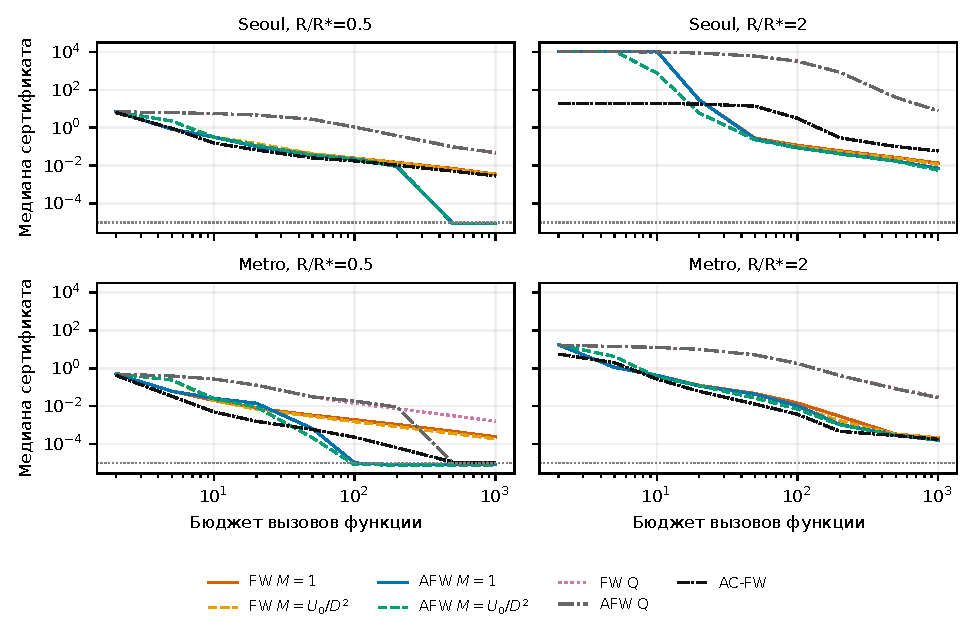
\includegraphics[width=\textwidth]{figures/count_comparators.pdf}
\caption{Медианы скалярных сертификатов по всем различным вершинам
при заданных бюджетах вызовов функции. Кривые включают неуспешные
запуски и оплаченную предварительную обработку AC-FW; завершённые
результаты переносятся вперёд. Горизонтальный пунктир — $10^{-5}$.
BT не получает кривизну, Q получает аналитические $H_0,H_1$.
Это парные конечные условия, а не доверительные полосы для
генеральной совокупности задач.}
\label{fig:counts}
\end{figure}

При активных радиусах обе инициализации AFW-BT сертифицируют каждый
старт за 1000 вызовов функции. FW-BT не сертифицирует ни одного
старта Seoul и лишь 2/24 или 3/24 на Metro. AC-FW даёт 13/24
успехов на активном Metro и ни одного на активном Seoul.
AFW-Q с известной кривизной успешен на всех активных стартах Metro,
но ни на одном активном Seoul, что иллюстрирует консервативность
аналитических параметров. При внутренних радиусах ни один метод
этого сравнения семи методов со скалярным сертификатом не достигает
цели за 1000 вызовов функции. Результаты к лимиту и медианы вызовов
с учётом цензурирования приведены отдельно в таблице~\ref{tab:counts}.

Эталоны отделяют оставшуюся ошибку от запаздывания остановки.
На внутреннем радиусе Metro у всех 24 стартов каждого BT-варианта
верхняя граница численной эталонной ошибки не больше $10^{-5}$
к исходному концу запуска, но у FW нет успехов по скалярному
сертификату, а у AFW лишь 6/24 или 7/24. На внутреннем Seoul
соответствующее условие эталонной ошибки выполняется у 12/30 и
18/30 AFW-стартов, хотя ни один скалярный BT-вариант не останавливается.
Следовательно, неуспех сертификата не равнозначен большой оставшейся
ошибке по функции.

\subsection{Контроль инициализации и единиц целевой функции}
Отдельное исследование $2\times2$ контролирует исходную точку против
обязательной вершины LMO и обновления AC против BT. Все четыре
условия оплачивают одинаковую обработку двух исходных точек,
сохраняют обе касательные границы и начинают первую пробу с одной
секущей кривизны. Лишь AC/вершина является исходным опубликованным
вариантом; остальные условия изолируют факторы. Исследование содержит
280 запусков на 70 прежних согласованных условиях и не вводит новых
наборов данных. Таблица~\ref{tab:init} показывает все три заданных
семейства с активным ограничением, включая неблагоприятное
масштабированное. Их конструкция и тождество запаса активной грани
даны в приложении~\ref{app:protocol}.

\begin{table}[htbp]
\centering\small
\caption{Контроль старта на трёх заданных семействах с активным ограничением, по десять согласованных экземпляров. Числа — сертифицированные старты за 1000 вызовов функции. O/V: исходная точка/обязательная начальная вершина LMO. Последний столбец — описательная парная медиана отношения сертификатов BT-V/AC-V и 95\%-й процентильный бутстреп-интервал, а не оценка ускорения.}
\label{tab:init}
\begin{tabular}{lrrrrl}
\toprule
Семейство & AC-O & AC-V & BT-O & BT-V & Отношение [интервал] \\
\midrule
active & 1 & 10 & 0 & 10 & 1.049 [0.935, 1.257] \\
active\_scaled & 0 & 0 & 0 & 0 & 1.530 [0.822, 1.750] \\
active\_highdim & 6 & 8 & 2 & 8 & 1.231 [0.798, 2.117] \\
\bottomrule
\end{tabular}
\end{table}

На семействе active смена старта повышает число успехов с 1 до 10
для AC и с 0 до 10 для BT. Описательный интервал отношения
сертификатов BT/AC при старте из вершины включает единицу.
Масштабированное семейство не решается ни одним из четырёх контролей.
Поэтому прежнее сравнение с вершинным стартом не изолирует преимущество
правила обновления.

Единицы целевой функции дают другой контроль. При
$\widetilde f=af+b$, $a>0$, умножение $M$ и $\varepsilon$ на $a$
сохраняет точные итераты, пробы и индекс остановки, поскольку
$G,U,L$ масштабируются вместе. Поэтому $M=U_0/D^2$ автоматически
эквивариантно; фиксация численного значения $M$ меняет эффективную
инициализацию. Отдельное исследование радиусов и масштабов на реальных
данных подтверждает счётчики во всех 60 парных сравнениях масштабов
для каждого метода с инициализацией по сертификату. Это элементарное
свойство не устанавливает более быстрый алгоритм.

\subsection{Причинные контроли остановки на фиксированных BT-траекториях}
Повторяются 432 исходные BT-траектории исследования счётных данных
с точным совпадением исходных концов и оракульных счётчиков.
Пять причинных мониторов дают 2160 зависимых профилей остановки.
Непересекающиеся блоки из $K=8,32,128$ оплаченных аффинных касательных
дают нижнюю оценку с одним дополнительным полным LMO на завершённый
блок; скалярная огибающая сохраняется. Отдельный стандартный контроль
получает $\mu=0.01$ и использует
$f-\norm{\nabla f}^2/(2\mu)$ как нижнюю оценку.
Приложение~\ref{app:monitors} доказывает корректность и раздельный
учёт оракулов; размеры блоков фиксируются до результатов, и ни один
монитор не читает эталон.

\begin{table}[htbp]
\centering\small
\caption{Раздельные причинные контроли на 432 точно повторённых BT-траекториях, дающие 2160 зависимых профилей. Используется первая остановка профиля или исходный лимит. Последний столбец сравнивает суммарные LMO направления и сертификата со скалярным профилем. Контроль с известным $\mu$ получает аналитический коэффициент регуляризации; блоки его не получают.}
\label{tab:monitors}
\begin{tabular}{lrrr}
\toprule
Профиль & Сертифицировано & Ранних префиксов & Больше LMO \\
\midrule
scalar & 129 & 0 & 0 \\
block\_8 & 129 & 0 & 432 \\
block\_32 & 129 & 0 & 425 \\
block\_128 & 129 & 0 & 380 \\
known\_mu & 226 & 110 & 0 \\
\bottomrule
\end{tabular}
\end{table}

Ни один проверенный блок не даёт более ранней остановки.
Контроль с известным $\mu$ даёт 226 успехов вместо 129 и 110 более
ранних префиксов, без дополнительных LMO, но с дополнительной
информацией о модели. На внутреннем Metro каждый BT-вариант теперь
достигает 24/24 успехов к исходному концу; оба AFW-варианта делают
это за 1000 вызовов функции. Внутренний Seoul остаётся трудным:
AFW даёт лишь 4/30 или 10/30 успехов к концу и ни одного за
1000 вызовов функции. Эти контроли не устанавливают адаптацию к
неизвестной сильной выпуклости и не оценивают точный двойственный
сертификат Фенхеля с усреднённым градиентом из~\cite{pedregosa}.
Они показывают, что наблюдаемая стоимость остановки — отдельный
практический вопрос.
